\section{Einleitung}
Ein großer Teil der Forschung in der Physik umfasst das Schreibenund Entwickeln umfangreicher Programmcodes. Diese werden meist über Jahre oder gar Jahrzehnte hinweg aufgebaut. Viele Codes werden von gro"sen Gruppen gemeinsam weiter entwickelt. Um Programmcode effizient zu dokumentieren und Änderungen auch Jahre später noch rückverfolgbar zu machen wurden Versionskontrollsysteme entwickelt. Diese Systeme sollen einen Überblick verschaffen über den Verlauf von Änderungen, aber auch die Zuordnung von Änderungen zu Personen ermöglichen. Mittlerweile nutzen fast alle Entwickler Git als Versionskontrolle. Dafür werden zumeist auch öffentliche Server (\url{Gitlab.com} oder \url{Github.com}) genutzt um den gesamten Code der Community zur Verfügung zu stellen\footnote{Der Quelltext dieser Arbeit steht auf Github zur Verfügung unter: {\url{https://github.com/tillhanke/git-basics}}}.

In dieser Arbeit sollen die Grundlagen der Arbeit mit Git erklärt werden. Der Fokus liegt dabei auf dem Arbeiten alleine mit einer dezentralen Sicherung des Codes. Zusätzlich wird am Ende auf die gemeinschaftliche Arbeit mit Git eingegangen.

Alle Instruktionen in dieser Arbeit beziehen sich auf Linux Betriebssysteme. Die meisten der angegebenen Befehle werden auch auf MacOS Systemen funktionieren. Git ist auch für Windows OS verfügbar jedoch wird darauf in dieser Arbeit nicht eingegangen. Auch wird die Installation von Git auf den genutzten Maschinen vorausgesetzt.

\subsection{Versionskontrolle}
Das Ziel einer Versionskontrolle wie Git ist es die Änderungen an einem Projekt zu dokumentieren. In Abb. \ref{fig:vers-kontrol}
ist eine solche Protokollierung visualisiert. Um Änderungen zu verfolgen werden zu jeder Änderungen Kommentare hinzugefügt - sogenannte "Commit-Messages". Diese Kommentare sollen das spätere zurückverfolgen der Änderungen vereinfachen. Um Speicherplatz zu sparen sollen in der Versionskontrolle möglichst nicht alle Dateien zu jedem Zeitpunkt gespeichert werden. Es wird somit nur einmal (zum Zeitpunkt der Erstellung) die komplette Datei gesichert. Danach werden von jeder Datei nur Informationen über die Änderungen abgespeichert.
\begin{figure}[!h]
    \centering
    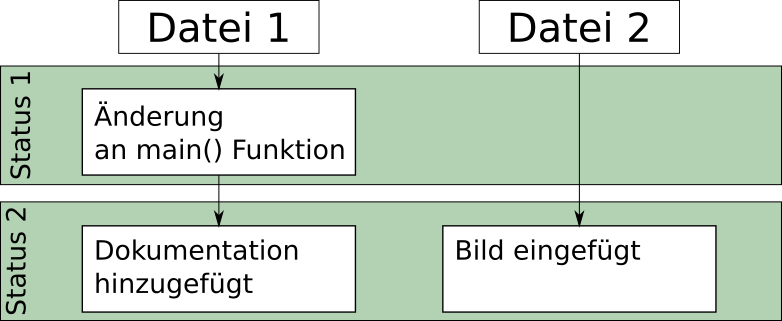
\includegraphics[width=0.9\textwidth]{Bilder/Versioncontrol.png}
    \caption{Beispiel Versionskontrolle von drei Änderungen an zwei Dateien desselben Projekts. Eingezeichnet sind zwei protokollierte Stadien des Projekts. Zu jeder Änderung ist ein Änderungskommentar angegeben.}
    \label{fig:vers-kontrol}
\end{figure}